\documentclass[a4paper,12pt]{article}
\usepackage{graphicx}
\usepackage{geometry}
\usepackage{fancyhdr}
\usepackage{hyperref}
\usepackage{array}

% Page layout settings
\setlength{\headheight}{14.5pt}
\geometry{top=1in, bottom=1in, left=1in, right=1in}

% Header and Footer settings
\pagestyle{fancy}
\fancyhf{}
\fancyhead[C]{Group 6}
\fancyfoot[C]{Page \thepage}

% Title page settings
\title{Lab Notebook}
\author{Group 6}
\date{\today}

\begin{document}

% Title Page
\begin{titlepage}
    \centering
    \vspace*{0.5in}
    
    {\Huge\bfseries Lab Notebook \\[0.2cm]}
    
\includegraphics[width=0.3\textwidth]{university_logo.png} \\[1.1cm]
    
    {\Large\bfseries Semester: 2 \\[0.5cm]}
    {\Large\bfseries Subject: Software Tools and Technology-I Lab \\[0.5cm]}
    {\Large\bfseries Group Number: 6 \\[0.5cm]}
    {\Large\bfseries Department: BCA and BSc \\[0.5cm]}
    
    {\Large \textbf{GitHub Repository:} \href{https://github.com/codeAtSin/group-6-final}{https://github.com/codeAtSin/group-6-final} \\[2cm]}
    
    \begin{tabular}{| l | c | c |}
        \hline
        \textbf{Name} & \textbf{Department} & \textbf{Roll Number} \\
        \hline
        Atul Sinha & BCA & 30001223022 \\
        \hline
        Neha Halder & BCA & 30001223046 \\
        \hline
        Arpan Singha Chowdhury & BCA & 30001223026 \\
        \hline
        Srija Saha & BSc & 30059223046 \\
        \hline
        Ankit Rai & BCA & 30001223060 \\
        \hline
    \end{tabular}

    \vfill

    {\large\bfseries MAKAUT \\ Information Technology}
\end{titlepage}

\newpage

% Table of Contents
\tableofcontents

\newpage

% Experiment/Assignment Section
\section{Assignment Details}
\textit{(Objective: To create a group lab book using \LaTeX \  and GitHub.)}
\begin{enumerate}
    \item Create a public Git repository.
    \item Add other members as collaborators.
    \item Push a LaTeX file in lab notebook format to the repository. The cover page should include:
    \begin{itemize}
        \item Each group member's name
        \item Roll number
        \item Department
    \end{itemize}
    \item Each member must write one lab notebook entry.
    \item Each member commits their entry to the Git repository.
\end{enumerate}

\newpage

% Individual Sections
{ \textbf{Date:} \today}
\section{Atul Sinha}

\subsection{Git Branching, Merging and Resolving conflicts}
In the given assignment I practiced git branching, merging and resolving the conflicts if any arrises.
\begin{enumerate}
    \item Created a new repository on GitHub named \texttt{git-advanced} then cloned it to my local machine.
    \item Created and switched to a new branch called \texttt{feature-1}.
    \item I created a file named \texttt{shared.txt} with the following content:
    \begin{verbatim}
    This is a shared file.
    Line 1: Original text.
    Line 2: Original text.
    \end{verbatim}
    \item Then staged and committed the file with a meaningful message to push it to GitHub.
    \item Created and switched to another branch called \texttt{feature-2}.
    \item Checked out the \texttt{shared.txt} file from the main branch, modified \texttt{shared.txt} to include.
    \begin{verbatim}
    Line 2: Modified text in feature-2.
    \end{verbatim}
    \item Staged and committed the changes with a meaningful message and pushed to GitHub.
    \item Switched back to the \texttt{feature-1} branch and modified \texttt{shared.txt} to include:.
    \begin{verbatim}
    Line 2: Modified text in feature-1.
    \end{verbatim}
    \item Staged and committed the changes with a meaningful message and then pushed to GitHub.
    \item Merged \texttt{feature-1} into the main branch.
    \item Merged \texttt{feature-2} into the main branch, which introduced a conflict.
    \item Then resolved the conflict by editing the file and committed the resolution.
    \item Finally pushed the updated main branch to GitHub.
    \item Then deleted the \texttt{feature-1} and \texttt{feature-2} branches.
\end{enumerate}
\href{https://github.com/codeAtSin/git-advanced}{CLICK: GitHub Repo for this assignment}
\par\vspace{2em}
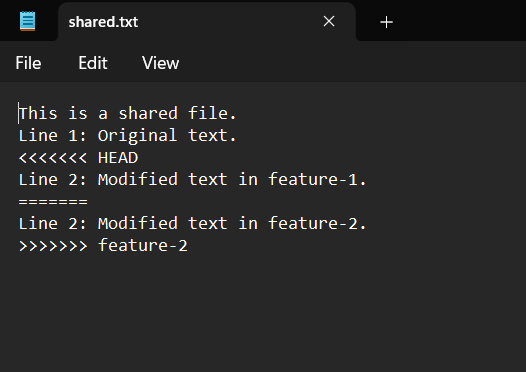
\includegraphics[width=0.8\textwidth]{conflictfile.png}
\par\vspace{2em}
\large\textbf{Showing conflicts in file.}
\par\vspace{2em}
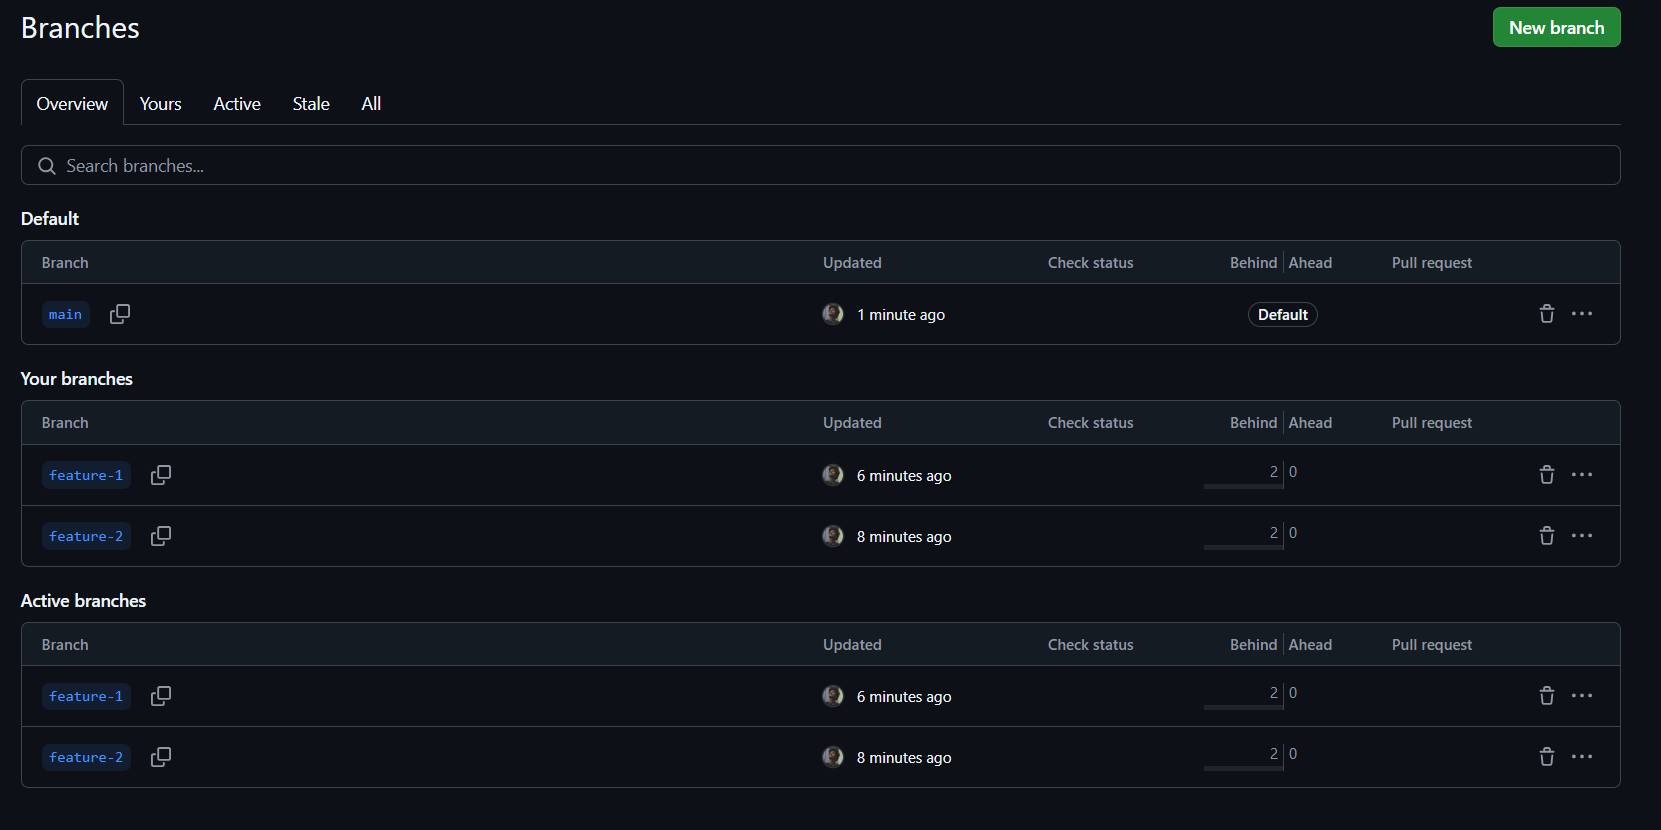
\includegraphics[width=0.7\textwidth]{allpushes.png}
\par\vspace{2em}
\large\textbf{Screenshots showing all the pushes in the repo.}
\vspace{0.3in}


\newpage
{ \textbf{Date:} \today}
\section{Neha Halder}

\subsection{Algorithm for Calculator in C Program}

Below is the algorithm I followed to create a basic calculator in C:

\subsubsection*{Algorithm}

\begin{enumerate}
    \item \textbf{Define Functions:} in C program
    \begin{itemize}
        \item \texttt{add(x, y)}: Returns \texttt{x + y}.
        \item \texttt{subtract(x, y)}: Returns \texttt{x - y}.
        \item \texttt{multiply(x, y)}: Returns \texttt{x * y}.
        \item \texttt{divide(x, y)}: Returns \texttt{x / y} or prints "Cannot divide by zero" if \texttt{y == 0}.
    \end{itemize}
    
    \item \textbf{Main Loop:}
    \begin{itemize}
        \item Display the menu with the following options: Add, Subtract, Multiply, Divide, Exit.
        \item \textbf{Get user choice:}
        \begin{itemize}
            \item If user inputs \texttt{5}, exit the program.
            \item Otherwise, prompt the user to input two numbers.
        \end{itemize}
        \item \textbf{Perform operation based on the user's choice:}
        \begin{itemize}
            \item Call the appropriate function and display the result.
        \end{itemize}
        \item Handle invalid inputs by printing "Invalid input."
    \end{itemize}
\end{enumerate}

\subsubsection*{Example Iteration}

\begin{enumerate}
    \item \textbf{User Chooses Operation:} User enters \texttt{1} for addition.
    \item \textbf{User Inputs Numbers:} User enters \texttt{12} and \texttt{8}.
    \item \textbf{Result Calculation:} \texttt{add(12, 8)} returns \texttt{20}.
    \item \textbf{Output:} Result is \texttt{20.0}.
    \item \textbf{User Chooses to Exit:} User enters \texttt{5}.
    \item \textbf{Program Ends.}
\end{enumerate}

\href{https://github.com/Nehaaa05/calculator/blob/main/calculator.c}{CLICK: GitHub Repo for Calculator}
\par\vspace{2em}
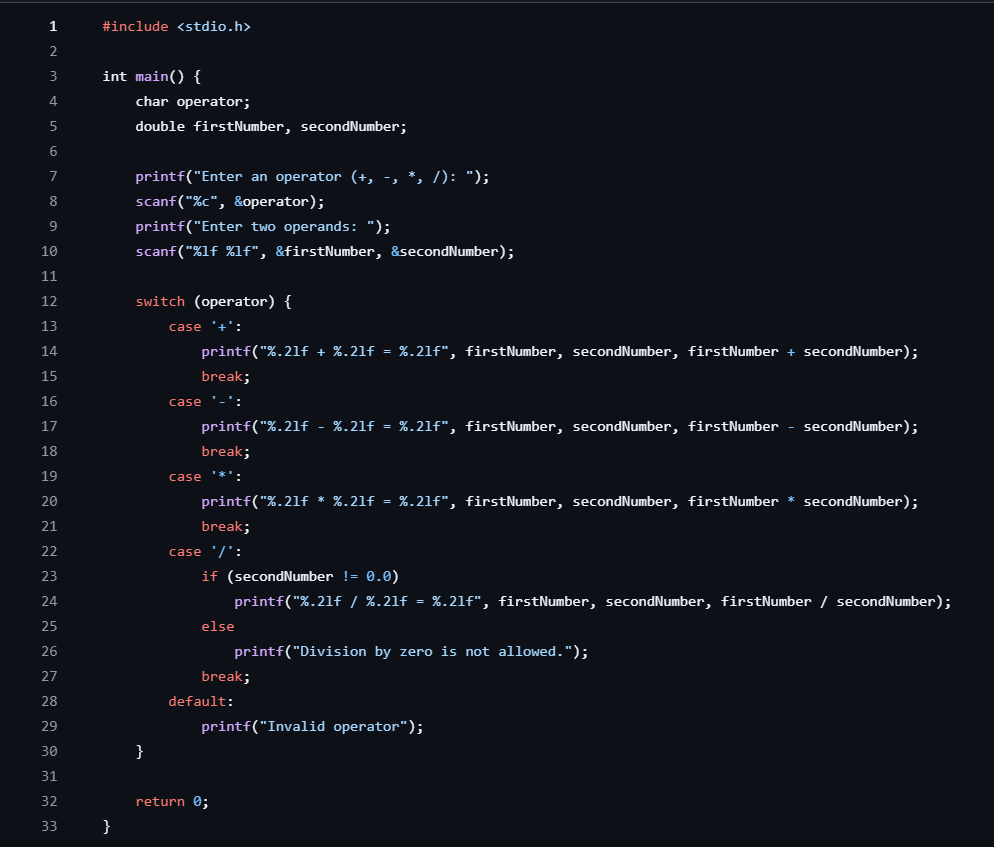
\includegraphics[width=0.7\textwidth]{ccalcula.png}
\par\vspace{2em}
\large\textbf{Screenshots showing the calculator code.}
\par\vspace{2em}
\vspace{0.3in}


\newpage
{ \textbf{Date:} \today}
\section{Arpan Singha Chowdhury}
\subsection{Document Class and Page Setup}
\begin{itemize}
    \item \texttt{\textbackslash documentclass[a4paper,10pt]\{article\}}: Defines the document as an A4 paper with a 10-point font size.
    \item \texttt{\textbackslash usepackage\{geometry\}}: Configures 1-inch margins on all sides.
\end{itemize}

\subsection{Packages Used}
\begin{itemize}
    \item \texttt{\textbackslash usepackage\{enumitem\}}: Enhances list formatting.
    \item \texttt{\textbackslash usepackage\{fancyhdr\}}: Customizes headers and footers.
    \item \texttt{\textbackslash usepackage\{parskip\}}: Adds space between paragraphs.
    \item \texttt{\textbackslash usepackage\{titlesec\}}: Customizes section titles.
\end{itemize}

\subsection{Header and Footer Customization}
\begin{itemize}
    \item \texttt{\textbackslash pagestyle\{fancy\}}: Applies the fancy page style.
    \item \texttt{\textbackslash fancyhf\{\}}: Clears default header and footer settings.
    \item \texttt{\textbackslash renewcommand\{\textbackslash headrulewidth\}\{0pt\}}: Removes the header rule.
    \item \texttt{\textbackslash renewcommand\{\textbackslash footrulewidth\}\{0pt\}}: Removes the footer rule.
\end{itemize}

\subsection{Document Content}
\begin{itemize}
    \item \textbf{Personal Information:} Includes date of birth, gender, marital status, and nationality.
    \item \textbf{Education:} Lists current education details.
    \item \textbf{Skills:} Enumerates programming and technical skills.
    \item \textbf{Hobbies:} Lists personal interests and activities.
    \item \textbf{Referees:} Notes that references are available upon request.
\end{itemize}
    
\subsection{End Document}
\begin{itemize}
    \item \texttt{\textbackslash end\{document\}}: Ends the document content.
    \end{itemize}

\includegraphics[width=0.8\textwidth]{arpancv.png}
\par\vspace{2em}
\large\textbf{The CV in pdf format.}
\par\vspace{2em}
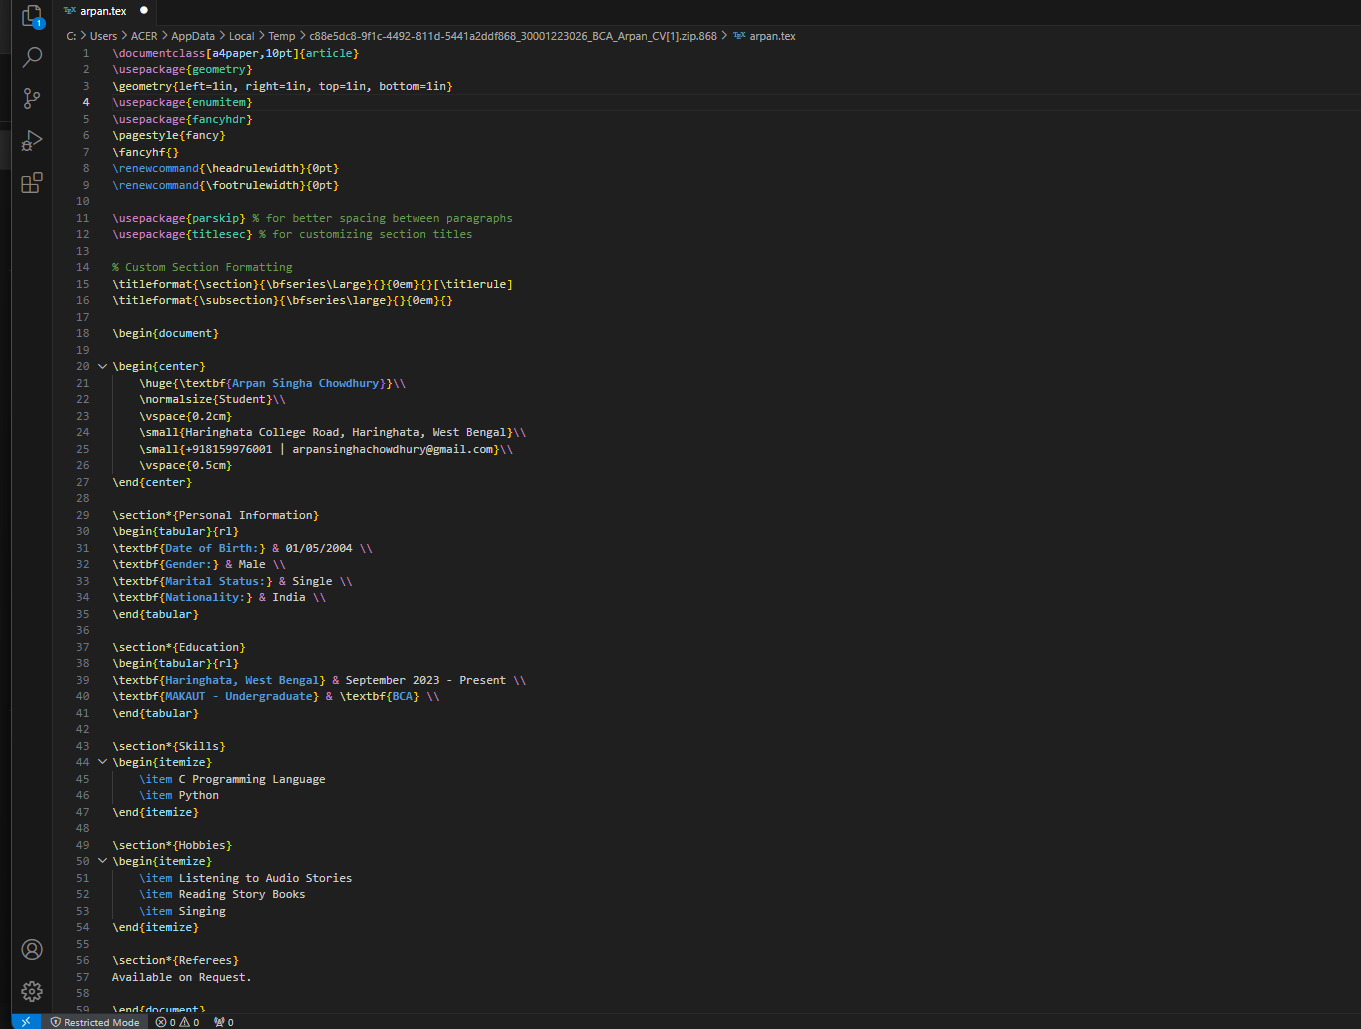
\includegraphics[width=0.9\textwidth]{arpancvtex.png}
\par\vspace{2em}
\large\textbf{Screenshots showing tex code for CV.}
\vspace{0.3in}
\newpage
{\textbf{Date :} \today}
\section{Ankit Rai}
\subsection{Assignment Completion Steps}

\begin{enumerate}
    \item \textbf{Clone the Repository:}
    \begin{itemize}
        \item Accessed the GitHub repository using the provided link: \url{https://github.com/GeekAyan/STT}.
        \item Cloned the repository to the local machine using GitHub Desktop.
        \item Followed the detailed run instructions in the `README.md` file to set up and run the application in the preferred IDE.
    \end{itemize}

    \item \textbf{Initial Observations:}
    \begin{itemize}
        \item Ran the application and noticed that the submit button appeared dull and unattractive.
    \end{itemize}

    \item \textbf{Modify Button Label:}
    \begin{itemize}
        \item Renamed the submit button to "Chin Tapak Dum Dum" to enhance its visibility and appeal.
    \end{itemize}

    \item \textbf{Fix Button Disproportions:}
    \begin{itemize}
        \item After renaming the button, observed that it became disproportionate in the application’s UI.
        \item Analyzed the button’s styling and layout properties to identify the cause of the disproportion.
        \item Adjusted the button’s font size and other UI settings to restore proportion and maintain a consistent appearance.
    \end{itemize}

    \item \textbf{Final Testing and Adjustments:}
    \begin{itemize}
        \item Ran the application again to ensure that the button was displayed correctly and functioned properly.
        \item Made any additional necessary UI fixes to ensure overall consistency and usability.
    \end{itemize}

    \item \textbf{Create Pull Request:}
    \begin{itemize}
        \item Committed the changes to the local repository.
        \item Pushed the updates to a new branch on the GitHub repository.
        \item Created a pull request to the original GitHub repository, detailing the changes made to the button and any other relevant UI adjustments.
    \end{itemize}
\end{enumerate}
\par\vspace{5em}
\large\textbf{Pull requests to the main repository :}
\par\vspace{2em}
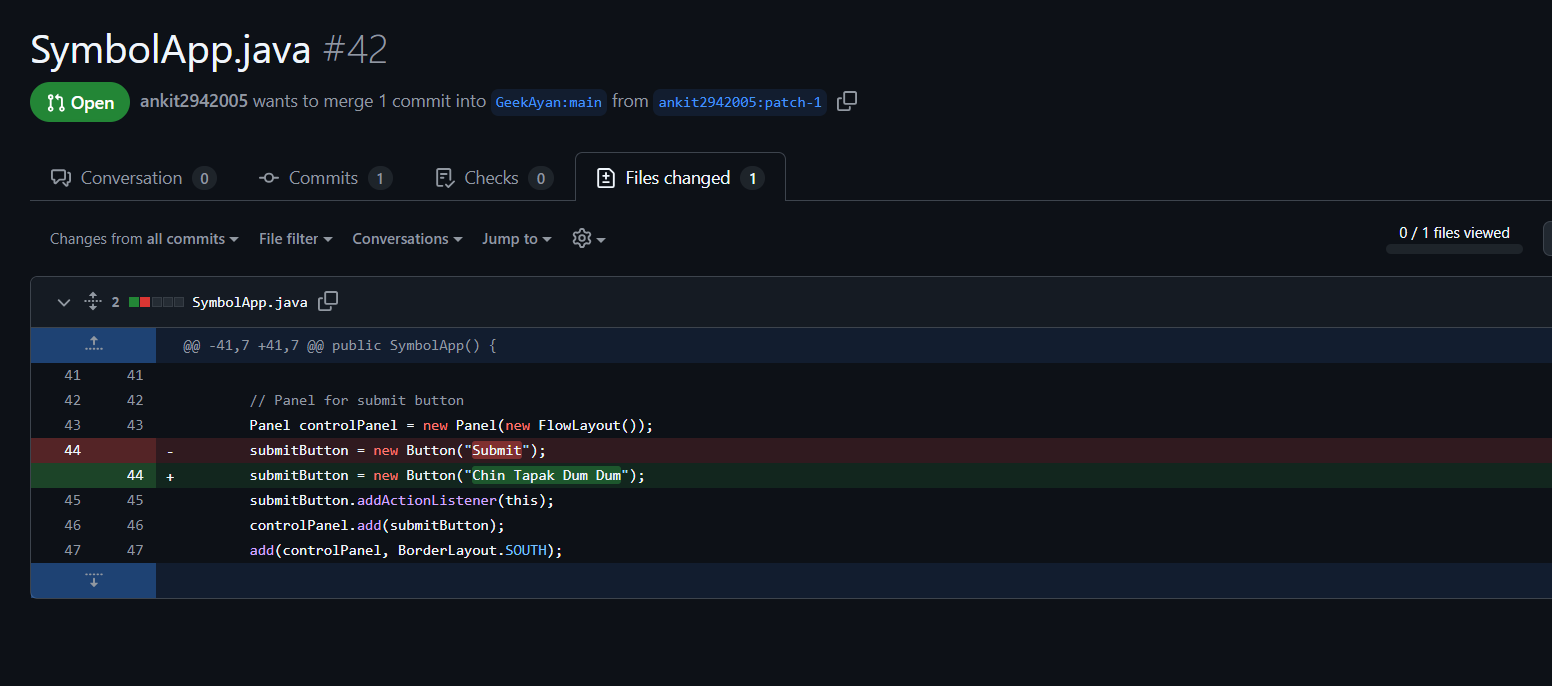
\includegraphics[width=0.9\textwidth]{ankit.png}
\par\vspace{2em}
\large\textbf{Screenshots showing pull request and the file changes made.}
\vspace{0.3in}
\newpage

{\textbf{Date :} \today}
\section{Srija Saha}

\subsection{A simple calculator program in C}
The Algorithm used to make the following calculator is : -
\begin{enumerate}
    \item \textbf{Start}
    \item \textbf{Show Menu}:
    \begin{quote}
        Display options for operations (\texttt{+}, \texttt{-}, \texttt{*}, \texttt{/}).
    \end{quote}
    \item \textbf{Get Operator}:
    \begin{quote}
        Read the chosen operator from the user.
    \end{quote}
    \item \textbf{Get Numbers}:
    \begin{quote}
        Prompt the user to enter two numbers.
    \end{quote}
    \item \textbf{Perform Calculation}:
    \begin{itemize}
        \item \texttt{+}: Add the numbers.
        \item \texttt{-}: Subtract the numbers.
        \item \texttt{*}: Multiply the numbers.
        \item \texttt{/}: Divide the numbers (handle division by zero).
    \end{itemize}
    \item \textbf{Show Result}:
    \begin{quote}
        Display the result of the operation.
    \end{quote}
    \item \textbf{End}
\end{enumerate}

\subsection{Output Workflow}

\begin{enumerate}
    \item \textbf{Show Menu}:
    \begin{quote}
        \texttt{Simple Calculator} \\
        \texttt{Choose an operation:} \\
        \texttt{+ for addition} \\
        \texttt{- for subtraction} \\
        \texttt{* for multiplication} \\
        \texttt{/ for division} \\
        \texttt{Enter your choice:}
    \end{quote}
    \item \textbf{User Input for Operator}:
    \begin{quote}
        Example: \texttt{+}
    \end{quote}
    \item \textbf{Prompt for Numbers}:
    \begin{quote}
        \texttt{Enter two numbers:}
    \end{quote}
    \begin{quote}
        Example Input: \texttt{8 5}
    \end{quote}
    \item \textbf{Show Result}:
    \begin{itemize}
        \item For addition: \texttt{Result: 13.00}
        \par\vspace{2em} \textbf{Other Cases} \par\vspace{1em}
        \item For subtraction: \texttt{Result: 3.00}
        \item For multiplication: \texttt{Result: 40.00}
        \item For division (with non-zero divisor): \texttt{Result: 1.60}
        \item For division (with zero divisor): \texttt{Error! Division by zero.}
    \end{itemize}
\end{enumerate}
\par\vspace{5em}
\large\textbf{Code shown in VS Code :}
\par\vspace{2em}
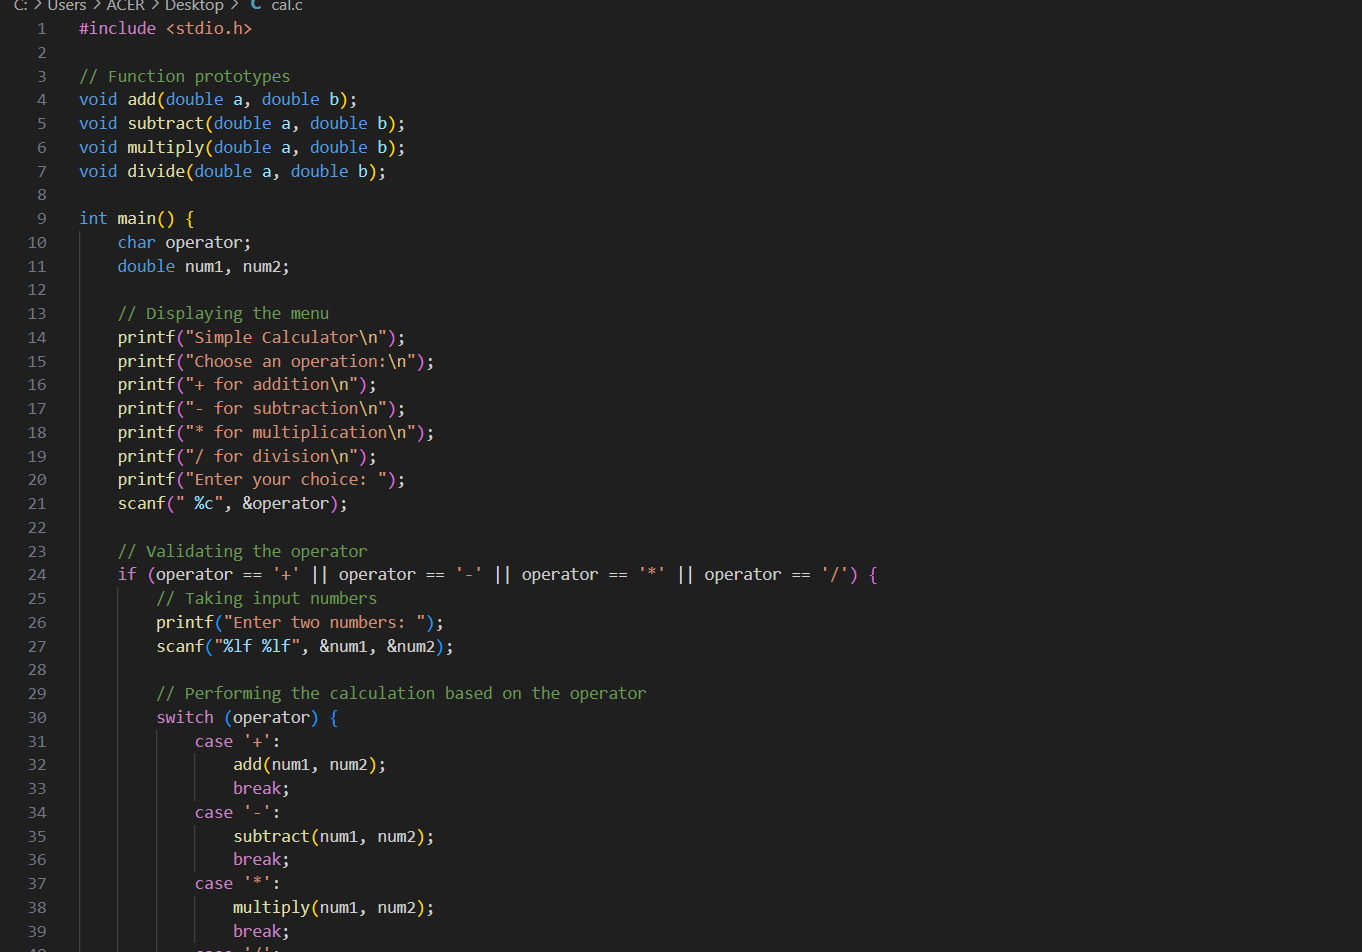
\includegraphics[width=0.8\textwidth]{srija.png}
\par\vspace{2em}
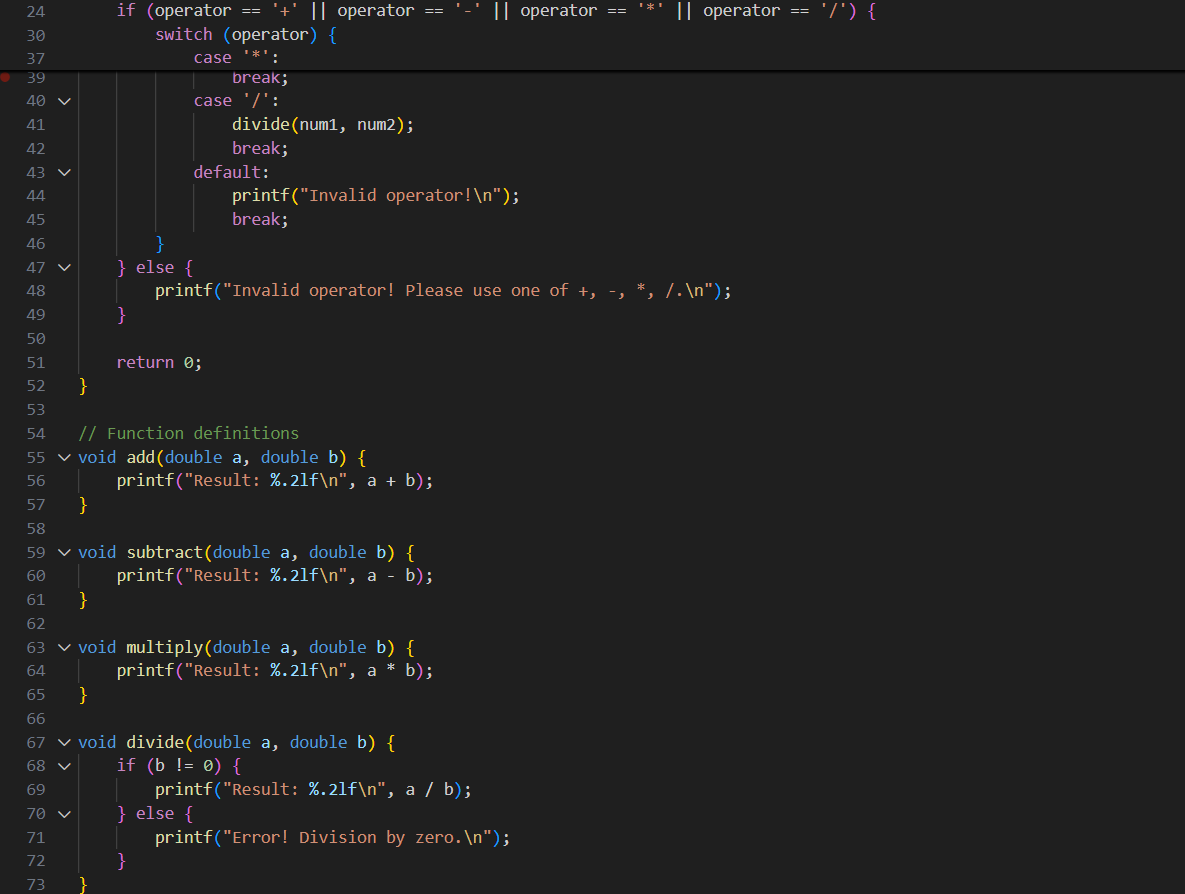
\includegraphics[width=0.8\textwidth]{srija1.png}
\par\vspace{2em}
\large\textbf{Screenshots showing code for the calculator}
\vspace{0.3in}
\end{document}